\documentclass{article}

    \usepackage[utf8]{inputenc}
    \usepackage[T1]{fontenc}
    \usepackage{aeguill}
    % \usepackage[francais]{babel}
    \usepackage[a4paper]{geometry}
    \usepackage{array}
    \usepackage{amsfonts}
    \usepackage{amsmath} 
    \usepackage{amssymb}
    \usepackage{amsthm}
    \usepackage{xspace}
    \usepackage{dsfont}
    \usepackage{collcell}
    \usepackage{datatool}
    \usepackage{enumitem}
    \usepackage{xstring}
    \usepackage{booktabs}
    \usepackage{environ}
    \usepackage{bbm}
    \usepackage{hyperref}
    \usepackage{graphicx}
    \usepackage{caption}
    \usepackage{stmaryrd}
    \usepackage[dvipsnames]{xcolor}
    \usepackage{tikz}
    \usetikzlibrary{trees}
    \usepackage{ulem}
    \usepackage{cancel}
    \usepackage{pgfplots}
    % \usepackage{minted}
    % \usemintedstyle{monokai}
    \usepackage{multicol}
    
    \pgfplotsset{compat=newest}
    \usetikzlibrary{automata} % LATEX and plain TEX
    \usetikzlibrary[automata] % ConTEXt
    \usetikzlibrary{arrows}
    \usetikzlibrary{automata,arrows,positioning,calc}
    \xdefinecolor{vertf}{named}{OliveGreen}
    \xdefinecolor{rougef}{named}{BrickRed}
    \xdefinecolor{bleuf}{named}{BlueViolet}
    \newcommand{\Var}{vecteur aléatoire réel\xspace}
    \newcommand{\var}{variable aléatoire réelle\xspace}
    \newcommand{\ssi}{si et seulement si\xspace}
    \newcommand{\cad}{c'est-à-dire\xspace}
    \newcommand{\fdr}{fonction de répartition \xspace}
    \newcommand{\pp}{\mathbb P}
    \newcommand{\un}{\mathbbm{1}}
    \newcommand{\esp}{\mathbb E}
    \newcommand{\vari}{\mathbb V}
    \newcommand{\cov}{\text{Cov}} 
    \newcommand{\gras}{\textbf}
    \newcommand{\itemb}{\item[$\bullet$]}
    \newcommand{\rouge}{\textcolor{red}}
    \newcommand{\bleu}{\textcolor{blue}}
    \newcommand{\rougef}{\textcolor{rougef}}
    \newcommand{\vertf}{\textcolor{vertf}}
    \newcommand{\bleuf}{\textcolor{bleuf}}
    \newcommand{\limn}{\underset{n\rightarrow +\infty}{\lim}}
    \newcommand{\flechn}{\underset{n\rightarrow +\infty}{\longrightarrow}}
    \newcommand{\RR}{\mathbb R}
    \newcommand{\Q}{\mathbb Q}
    \newcommand{\N}{\mathbb N}
    \newcommand{\Z}{\mathbb Z}
    \newcommand{\R}{\mathbb R}
    \newcommand{\D}{\mathbb D}
    \newcommand{\C}{\mathbb C}
    \newcommand{\Rn}{\mathbb R^n}
    \newcommand{\Rp}{\mathbb R^p}
    \newcommand{\Rq}{\mathbb R^q}
    \newcommand{\brn}{\mathcal B(\mathbb R^n)}
    \newcommand{\brp}{\mathcal B(\mathbb R^p)}
    \newcommand{\brq}{\mathcal B(\mathbb R^q)}
    \newcommand{\br}{\mathcal B(\mathbb R)}
    \newcommand{\brbarre}{\mathcal B(\overline{\mathbb R}}
    \newcommand{\pps}{P-presque-sûrement\xspace}
    \newcommand{\mespos}{\mathcal M^+(\mathcal B(\mathbb R^n),\mathcal B(\overline{\mathbb R}))}
    \newcommand{\cvps}{\xrightarrow[n\rightarrow\infty]{p.s.}}
    \newcommand{\cvld}{\xrightarrow[n\rightarrow\infty]{L^2}}
    \newcommand{\cvlp}{\xrightarrow[n\rightarrow\infty]{L^p}}
    \newcommand{\cvp}{\xrightarrow[n\rightarrow\infty]{\mathbb P}}
    \newcommand{\cvloi}{\xrightarrow[n\rightarrow\infty]{\mathcal L}}
    \newcommand{\definition}{\vspace{0.5cm}\begin{tcolorbox}[colback=bleuf!5!white,colframe=bleuf!75!black,title=Définition]}
    \newcommand{\propriete}{\vspace{0.5cm}\begin{tcolorbox}[colback=bleuf!5!white,colframe=bleuf!75!black,title=Propriété]}
    \newcommand{\proprietee}{\vspace{0.5cm}\begin{tcolorbox}[colback=red!5!white,colframe=red!75!black,title=Propriété]}
    \newcommand{\theoreme}{\vspace{0.5cm}\begin{tcolorbox}[colback=red!5!white,colframe=red!75!black,title=Théorème]}
    \newcommand{\lemme}{\vspace{0.5cm}\begin{tcolorbox}[colback=red!5!white,colframe=red!75!black,title=Lemme]}
    \newcommand{\proposition}{\vspace{0.5cm}\begin{tcolorbox}[colback=red!5!white,colframe=red!75!black,title=Proposition]}
    \newcommand{\fin}{\end{tcolorbox}\vspace{0.5cm}}
    \newcommand{\preuve}{\noindent\uline{Preuve :}\xspace}
    \newcommand{\remarque}{\noindent\uline{Remarque :}\xspace}
    \newcommand{\exemple}{\noindent\uline{Exemple :}\xspace}
    \newcommand{\rappel}{\noindent\uline{Rappel :}\xspace}
    \newcommand{\notation}{\noindent\uline{Notation :}\xspace}
    
    
    % transposition de tableaux
    
    
    \usepackage{booktabs,array}
    \def\Midrule{\midrule[\heavyrulewidth]}
    \newcount\rowc
    
    \makeatletter
    \def\ttabular{%
    \hbox\bgroup
    \let\\\cr
    \def\rulea{\ifnum\rowc=\@ne \hrule height 1.3pt \fi}
    \def\ruleb{
    \ifnum\rowc=1\hrule height 1.3pt \else
    \ifnum\rowc=6\hrule height \heavyrulewidth 
       \else \hrule height \lightrulewidth\fi\fi}
    \valign\bgroup
    \global\rowc\@ne
    \rulea
    \hbox to 10em{\strut \hfill##\hfill}%
    \ruleb
    &&%
    \global\advance\rowc\@ne
    \hbox to 10em{\strut\hfill##\hfill}%
    \ruleb
    \cr}
    \def\endttabular{%
    \crcr\egroup\egroup}
    
    
    
    \usepackage{tcolorbox}
    
  
    \hypersetup{colorlinks=true,linkcolor=black}
    
    \usepackage{fancyhdr}
    \pagestyle{fancy}
    \lfoot{S. DO, L. ZANINI }
    \rfoot{\thepage}
    \cfoot{ }
    \lhead{COMPRESSED SENSING PROJECT}
    \chead{}
    \rhead{}
    
    \renewcommand{\footrulewidth}{1pt}
    
    \newcommand{\ind}{\setlength\parindent{0.5cm}} 
    
\begin{document}
    
    \begin{titlepage}
    \begin{flushright}
    
\includegraphics{logo-ensae.jpg}
    \end{flushright}
    \vspace*{\stretch{0.5}}
    \hrulefill
    \begin{center}\Huge
    % End-to-end Multilingual 
    Compressed Sensing Project \\ 
    \textit{\Large A compressed sensing view of unsupervised text embeddings  }
    \end{center}
    \hrulefill
    \vspace*{1cm}
    \begin{center} \Large
    Salomé Do, Lucas Zanini
    \end{center}
    \vspace*{\stretch{1}}
    \begin{flushright}
    March, 22nd 2019
    \end{flushright}
    \end{titlepage}
    
\newpage
% % \thispagestyle{empty}
% \section*{Acknowledgements}
% \newpage 

\newpage
% \thispagestyle{empty}
\section*{Introduction}

Text documents have been, until recently, an underexploited
source of information due to their complex, non-numerical
structure. Low level natural language processing (NLP)
tasks as text classification, 
sequence tagging (POS-tagging, named entity recognition, ...) and 
parsing have long been tackled through bag-of-words methods 
and hidden markov models. The application of deep learning 
to NLP tasks (started around 2010s) has opened new, complementary 
and effective ways to solve these problems, eventually leading to core
innovations in high-level tasks such as question answering or 
language generation. Using feed-forward networks 
to generate low-dimensional representation of sparse, high 
dimensional word vectors; recurrent neural networks as LSTMs
to fit the sequential nature of sentences; and later on attention mechanims,
deep learning techniques have set new baselines on traditional benchmarks. 
However, the efficiency of these results is totally empirical 
and is not backed by theoretical results, in addition to having 
high computationnal costs. The article studied in this project \cite{arora2018sensing}
aims at giving some results on unsupervised text embeddings. 
\\ \\
To do so, it focusses on a compressed sensing view of the text 
embedding problem, which aims at provinding low-dimensional representation
for texts. As words can be viewed 
as very sparse vectors in the vocabulary space, providing a 
low-dimensional representation of a text can be seen as measuring 
words signals in a compressed way. The article explores this idea, 
and links compressed sensing to some LSTMs-learned text representations.
In order to evaluate such representations (through their 
performances on text classification), authors
 adapts a result in \cite{Calderbank2009CompressedL} on the quality
of low-dimensional compressed sensing representations as inputs
for a classification problem. \\ \\
In this work, we will first recall what are words and text embeddings, 
in order to recall the basic NLP background for a non-specialized reader,
and we will present author's text embeddings.
Then, we will focuss on the core part of this project : the compressed 
sensing part, and its application in text embeddings. Finally, we 
will present a reproduction of author's results, and discuss their
 statings and their implications.


\newpage 

\tableofcontents
\newpage

\section{Text embeddings}

A text embedding is a vector representing a text. Usually, 
we want this representation to be low-dimensional, and to 
keep some information on the meaning of the text. By necessity, 
these representations are generally unsupervised : it would be 
hard to define a "standard" representation to be learned in a 
supervised way. In this section, we recall usual ways to 
learn to generate word embeddings - upon which lie LSTMs text embeddings -, 
text embeddings, and we explain in which ways they can be used for 
tasks as text classification.


\subsection{Word embeddings}

The very beginning of most popular
text embeddings is word embeddings. In this part
we will briefly explain how such embeddings are learned, and we will
set the definitions and the general context for the rest of the 
work. \\ \\
Supposing that we have a vocabulary 
$\mathcal{V} = \{w_1, ..., w_V \}$, of size 
$| \mathcal{V} | = V$, a natural vector representation of any word 
$w_i, i=1, ..., V$ is the following :
\begin{align*}
    w_i &= 
    \left (
    \begin{array}{c}
        0 \\
        \vdots \\
        0 \\
        1 \\
        0 \\
        \vdots \\
        0 \\
    \end{array}
    \right ) \leftarrow i,\ \ \ w_i \in \R^V
\end{align*}

The problem with this simple representation is the dimension ($V$)
and its sparsity ($||w_i||_0 = 1, \forall i= 1, ..., V$) of the vectors.
To adress this issue, many techniques have been proposed, especially 
in recent deep learning developments. Non-deep learning techniques 
are based on co-occurence matrices : 
given a set $\mathcal{D}$ of
documents, we first build a matrix containing the number of co-occurrences
of every word in all documents in a context window of size $c$, 
for instance :
\begin{align*}
    M&=
    \left (
    \begin{array}{ccc}
        C(w_1, w_1) & \dots & C(w_1, w_V) \\
            \vdots    & \ddots&   \vdots       \\
        C(w_V, w_1) & \dots & C(w_V, w_V) \\
    \end{array}
    \right ) \in \R^{V\times V}
\end{align*} 
Where $C(w_i, w_j)$ is the number of times that the word $w_j$ appears 
in the context of $w_i$, the context being defined as the 
words far from at most $c$ words from $w_i$ in any of the documents
in $\mathcal{D}$. This matrix is usually regularized using 
positive pointwise mutual information (PPMI). A word $w_i$
is then represented as the $i$-th line of $M$, or its
PPMI counterpart. However, this representation does not get rid
of dimension neither sparsity problems. Assuming the PPMI
matrix is very sparse, we use, as it is frequently
done in high-dimensional statistics,
a singular value decomposition $M^{\text{PPMI}} = W \times D \times C$, 
keeping only the $k$
most important singular values and vectors, leading to a new truncated
version of $W$, of size $V\times k$, which becomes the embedding
matrix, each line being a word's embedding. This decomposition
has good denoising and generalization properties. \\ \\
In parallel, the most popular deep learning embedding
is the Word2Vec embedding, proposed in \cite{NIPS2013_5021}. This 
embedding is learned by trying to predict a word from its context 
(CBOW), or vice versa to predict a context from a given word 
(skip-gram); using a 1-hidden layer feed-forward neural network
(Figure \ref{skip-arch}). 

\begin{center}
    \captionof{figure}{Skip-gram architecture for Word2Vec}
    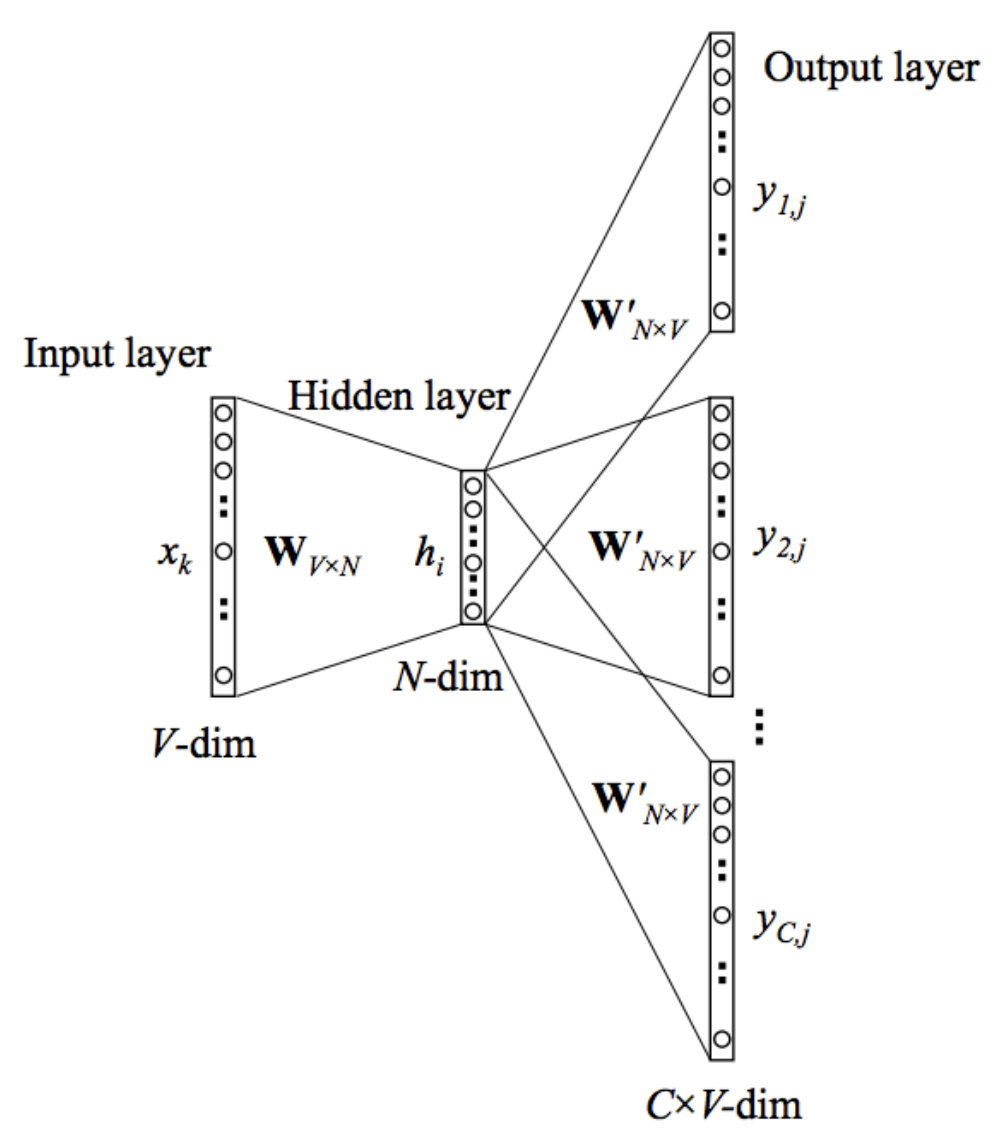
\includegraphics[scale=0.4]{skip-arch}
    \label{skip-arch}
\end{center}
Using some regularization and computationnal tricks during the training,
as replacing the softmax output function computation by a 
hierarchical softmax computation, or as using negative sampling loss
as an objective function, or doing frequency subsampling; which are 
detailed in \cite{Mikolov2013}; Word2Vec embeddings achieved better 
generalization and denoising properties than SVD. The main 
idea behind both Word2Vec and SVD embeddings, which makes them 
coherent as a good semantic representation, is called 
the distributionnal hypothesis. This linguistic hypothesis is built upon
Firth's statement that \textit{"a word is characterized by the 
company that it keeps"}. Thus, words employed in similar contexts
are more likely to have similar meanings. However, latest deep learning 
developments seem to have abandoned this approach, replaced by language modelling
as in \cite{howard2018universal, Peters_2018, devlin2018bert}, which 
are outside the scope of this project. \\ \\
The evaluation of such embeddings is difficult, as they are learned in an 
unsupervised way. However, two techniques are generally used to assess
embeddings representation quality : the evaluation of the embedding through
a downstream task, i.e. for instance the evaluation of classic text classifiers 
using the evaluated embedding as an input; and an evaluation through 
word similarities, with the objective that near vectors (regarding 
cosine distance) represent words with similar meanings. This evaluation
techniques are used in the same manner for text embeddings.

\subsection{From word embeddings to text embeddings}

In natural language processing, and more specifically in 
high-level tasks, there is no interest on studying single words. 
Thus, a natural question when working on texts, is : how to 
transform word embeddings to a single text embedding? In this section
we will describe 'natural' text embeddings, resembling the co-occurence
matrix described above, used in the article; and LSTMs embeddings, 
which are now more commonly used.

\subsubsection{Bag of n-Grams/Cooccurrences}

In this part, we will suppose that we have a vocabulary 
$\mathcal{V} = \{ v_1, ..., v_V\}$ and a document $d=w_1, ..., w_T$, 
where $w_i \in \mathcal{V}$ for any $i=1, ..., T$, and a fixed integer 
$n\in \N$. We recall 
that a $n$-gram is a sequence of $n$ words, 
for instance the set of unigrams is $\{v_1, ..., v_T \}$, the set 
of bigrams is $\{(v_1,v_2), (v_2, v_3), (v_1, v_3) ..., (v_{V-1}, v_V) \}$, etc.
We let $V_k$ be the number of possible $k$-grams over $\mathcal{V}$,
independently of order ($V_1 = V$), and 
$V_n^{\text{sum}} = \sum_{k=1}^n V_k$.\\ \\
For any $k\in \N$, let $B_k$ be a vector indicating, 
for any possible $k$-gram over $\mathcal{V}$, the number 
of occurences of this $k$-gram in the document.
A Bag-of-$n$-Grams, denoted $x^{\text{BonG}}$ is the concatenation of all the $B_k$ vectors
for $k = 1, ..., n$ : 
\[
x^{\text{BonG}} = [B_1, ..., B_N]\]
In order to simplify and get rid of order in the n-grams, author
merge the $k$-grams in the vocabulary that are the same words in a 
different order. Then, we can write :
$B^{\text{Co-oc}}_k = \sum_{t=1}^{T-k+1} e_{ \{w_t, ..., w_{t+k-1}\}  }$. 
A Bag-of-$n$-Co-occurrences (BonC) is then :

\[
x^{\text{BonC}} = [B^{\text{Co-oc}}_1, ..., B^{\text{Co-oc}}_N]\]

These embeddings are sparse, $V_n^{\text{sum}}$-dimensional vectors.


\subsubsection{DisC embeddings}
This document embeddings relies on word embeddings. 
Supposing that we have learned word embeddings and that we denote
$x_{v_i} \in \R^d, d<<V$ the embedding of the word $v_i \in \mathcal{V}$, for any
$i=1,..., n$; and that we still have our document $d= w_1, ..., w_T$; 
then the unigram embedding of the document is :
\[z^u = \sum_{t=1}^T x_{w_t}\]
$z^u$ can be re-written as the product of a compression matrix $A$ 
in which columns are word embeddings $x_w$; and the "Bag-of-1-grams" document embedding : 

\[z^u = Ax^{\text{Bo1G}} = \sum_{t=1}^T A e_{w_t} = \sum_{t=1}^T x_{w_t} \]
Authors extend this unigram definition to $n$-co-occurrences by using
element-wise multiplication of word embeddings, defining: 
\[\tilde{x}_{\{w_1, ..., w_n\}} = d^{(n-1)/2} \odot_{t=1}^n x_{w_t} \ \ \in \R^d \]
Then, DisC (distributed co-occurence) embeddings are defined as
the concatenation of:

\[
    z^{(n)} = \left [ 
                C_1 \sum_{t=1}^T \tilde{x}_{w_t}, 
                ..., 
                C_n \sum_{t=1}^{T-n+1} \tilde{x}_{\{w_t, ..., w_t+n-1\}}
              \right ]
              \in \R^{nd}
\]
With $C_1,..., C_n$ being scaling factors, detailed later. As in the 
unigram case, DisC embeddings are directly related to compressed sensing
as we can find $A^{(n)}\in R^{dn \times V_n^{\text{sum}}}$ such that:
\[z^{(n)} = A^{(n)}x^{BonC} \]


\subsubsection{LSTMs}

LSTMs, which stands for Long-Short-Term Memory are a kind of recurrent
neural networks, introduced in \cite{Hochreiter:1997:LSM:1246443.1246450}.

\subsection{Why text embeddings? }




\newpage
\section{Text embedding as a Compressed Sensing problem}

\subsection{Results on compressed sensing for classification}


\subsection{Links with LSTMs}

\subsection{Sparse recovery with pretrained embeddings}





\newpage
\section{Experiments and discussion}

\subsection{Results reproduction}

\subsection{Testing DisC embeddings on real life data}


\subsection{Discussion}



\bibliography{references} 
\bibliographystyle{ieeetr}
\end{document}